\section{Introduction}


Fourier series (FS) gives a new idea to expand a continuous and periodic signal with a series of trigonometric functions, which glanced at frequency analysis at the first time. Based on the idea of FS, other transformations were proposed to extend the limit on FS: (1) Fourier transform (FT) for continuous but non-periodic signals; (2) discrete time Fourier transform (DTFT) for sampled signals; (3) discrete Fourier transform (DFT) for completely discrete analysis. These transformations make up Fourier transform family under Dirichlet conditions. Besides, Laplace transform extends the frequency into complex domain and Z transform simplifies DTFT practically.


Analysis in frequency domain provides more options to process signals or evaluate linear systems. For example, a spectrum given by fast Fourier transform (FFT, the fast algorithm for DFT) shows the frequency distribution of the signal; the location of poles and zeros of a system demonstrate the stability and dynamic properties.


In this report, attentions are paid to digital signal processing. Power spectrum density is firstly introduced as a tool for frequency analysis and a new algorithm is delivered. Then the design and properties of some common used filters are discussed. Finally, an example is given to show processing procedure and the results.




\section{Power Spectrum Density}


DFT is used to analysis a certain signal. However, there are many kinds of stochastic signals whose statistical properties are the most concerned. As for a stationary and random signal, power spectrum density (PSD) is taken to estimate its properties in frequency domain.


PSD is defined as the Fourier transform of the autocorrelation function of the given signal $x(t)$
\begin{equation}
    S_x(\omega) = \mathscr{F}\left(R_{xx}(\tau)\right) = \int_{-\infty}^{+\infty} R_{xx}(\tau) \iexp{-\mathrm{j} 2 \uppi \omega \tau} \diff \tau
\end{equation}
where the autocorrelation function $R_{xx}(\tau)$ is 
\begin{equation}
    R_{xx}(\tau) = \lim_{T\to \infty} \frac{1}{2T}\int_{-T}^{T} x(t) x(t-\tau)  \diff t
\end{equation}
Thus, the PSD is computed by
\begin{align}
    S_x(\omega) &= \int_{-\infty}^{+\infty} \left(\lim_{T\to \infty} \frac{1}{2T}\int_{-T}^{T} x(t) x(t-\tau)  \diff t t\right) \iexp{-\mathrm{j} 2 \uppi \omega} \diff \tau \notag \\ 
    &= \lim_{T\to \infty} \frac{1}{2T} \int_{-T}^{T} x(t)\iexp{-\mathrm{j} 2 \uppi \omega t} \left( \int_{-\infty}^{+\infty} x(t-\tau) \iexp{-\mathrm{j} 2 \uppi \omega \left(\tau-t\right)} \right) \diff t \notag \\
    &= \lim_{T\to \infty} \frac{1}{2T} \int_{-T}^{T} x(t)\iexp{-\mathrm{j} 2 \uppi \omega t} X^*(\jomega) \diff t \notag \\
    &= \lim_{T\to \infty} \frac{1}{2T} X(\jomega) X^*(\jomega) \notag \\
    &= \lim_{T\to \infty} \frac{1}{2T} \left| X(\jomega) \right|^2
        \label{eq:psd}
\end{align}
Eq~\eqref{eq:psd} is also known as Wiener–Khinchin theorem, which demonstrate the relationship between PSD and general frequency spectrum.




\subsection{Classical Power Spectrum Density Estimation}


Analog signals are analyzed based on the sampled data. Two important effects should be considered in sampling: (1) sampling should satisfy Nyquist sampling theorem, where the sampling frequency should be at least twice the maximum frequency of the origin signal. In practice, an analog anti-aliasing filter is usually used before the signal is sampled. (2) Finite sampling is equivalent to applying a window function to the infinite signal, which leads to frequency leakage effect. Because of these two effects, the PSD computed from the sampled data is just the estimation of the PSD of origin analog signal. That's why we usually say `spectrum estimation' instead of `spectrum calculation'.


The most direct method to estimate PSD is to discretize Eq~\eqref{eq:psd} using DFT and cancel the limit as below.
\begin{equation}
    S_x(\omega) \approx \frac{1}{T} \left| X(k) \right|^2 = \frac{1}{Nf_s} \left| X(k) \right|^2
\end{equation}
where $T$ is the total time of data, $N$ is the total number of points, $f_s$ is the sampling frequency. $X(k)$ is the DFT of $x(n)$, given by
\begin{equation}
    X(k) = \sum_{n=0}^{N-1} x(n) \iexp{-\mathrm{j} 2 \uppi \frac{n}{N}k} \label{eq:DFT}
\end{equation}
In the case where a window function $w(n)$ is applied to the sampled data, the PSD should be normalized as below.
\begin{equation}
    S_x(\omega) = \frac{1}{\sum_{n=0}^{N-1} w^2(n) f_s} \left| X(k) \right|^2 \label{eq:periodogram}
\end{equation}


PSD can be estimated by combining Eq~\eqref{eq:DFT} and Eq~\eqref{eq:periodogram}. This direct method is called `periodogram'. Both MATLAB and Python provide built-in function to calculate the periodogram named respectively \verb|periodogram| and \verb|scipy.signal.periodogram|. 


An example for PSD estimation is shown in Fig~\ref{fig:plotPSD}. The result of periodogram looks very noisy, especially in high frequency band. To improve the accuracy of the estimation, Welch proposed a method to estimate PSD by dividing the data into overlapped segments and computing the average of the periodogram of each segment.


\begin{figure}[!htb]
    \centering
    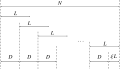
\includegraphics[width=0.5\textwidth]{Welch.pdf}
    \caption{The idea of Welch's method to estimate PSD.}
    \label{fig:Welch}
\end{figure}


The idea of Welch's method is shown in Fig~\ref{fig:Welch} and the relevant functions are \verb|pwelch| in MATLAB and \verb|scipy.signal.welch| in Python. 




\subsection{Logarithmic Frequency Axis Power Spectral Density}


As shown in Fig~\ref{fig:plotPSD}, by averaging PSD using Welch's method, the curve is less noisy. However, because the data is divided into segments, the length decreases, which decreases the frequency resolution. To further improve Welch's method, a new method named Logarithmic frequency axis Power Spectral Density (LPSD) was proposed \cite{trobsImprovedSpectrumEstimation2006}.



\begin{figure}[!htb]
    \centering
    \includegraphics[width=0.7\textwidth]{plotPSD.pdf}
    \caption{Comparison of three methods to estimate PSD.}
    \label{fig:plotPSD}
\end{figure}


\section{Filter Design}





\subsection{Common Used Filters}
% continus/discrete, FIR/IIR
% butter/... (functions)




\subsection{Zero-Phase Filtering}
% phase compensator
% flip/filter...




\section{Results}
% example




\section{Conclusions}





